\begin{justify}
\chapter[Resultados]{Resultados}
\label{ch:resul}
\section{Definición de Variables y Parámetros}
Para el desarrollo del modelo de simulación es necesario acotar el sistema a simular a los objetivos centrales del proyecto para así evitar perder el foco deseado por realizar un modelo complejo. Dado que el fin de esta simulación es simular el comportamiento físico de los dispositivos LoRa, algunos datos que en condiciones reales son variables serán tomadas como parámetros estáticos con el fin de simplificar el modelo de simulación. Los valores asignados a estas variables, fueron obtenidos en la guía del desarrollador para dispositivos LoRa de la empresa Orange, estos datos son escogidos dado que múltiples investigadores~\cite{Juha} al realizar pruebas empíricas usaron estos mismos datos como base para sus investigaciones con los dispositivos LoRa, obteniendo resultados muy cercanos a los que entrega la especificación de LoRa.Los parámetros constantes de este sistema a modelar son los siguientes:
\begin{itemize}
\item $Coding Rate=\frac{4}{5}$
\item $Ancho de Banda=125KHz$
\item $Packet Error Rate (PER)=1\%$
\item $Gateway Data Bit Rate Inicial=300bps$
\end{itemize}
\newpage
\noindent
En relación a los parámetros fijos para el modelo de simulación, se aprecia en Tab~\ref{tab:par} se han definido algunos valores fijos para variables dependientes de los Spreading Factor a usar en la etapa de ADR de la comunicación LoRa~\cite{orange}.
\begin{table}[!ht]
\centering
\begin{tabular}{|c|c|c|c|}
\hline
Spreading Factor & Bit rate & Alcance de Transmisión & Time on Air\\ \hline
SF7 & $5470bps$ & $2km$ & $56ms$ \\ \hline
SF8 & $3126bps$ & $4km$ & $100ms$ \\ \hline
SF9 & $1760bps$ & $6km$ & $200ms$ \\ \hline
SF10 & $980bps$ & $8km$ & $370ms$ \\ \hline
SF11 & $440bps$ & $11km$ & $740ms$ \\ \hline
SF12 & $290bps$ & $14km$ & $1400ms$ \\ 
\hline
\end{tabular}
\caption{Asignación de Valores para los diferentes Spreading Factor}
\label{tab:par}
\end{table}

\section{Definición de Fases de Transmisión en LoraWAN}
Para que exista comunicación entre los nodos y Gateway LoRa deben ejecutar fases de comunicación, las que dan inicio a eventos, como el envío de un mensaje o el cambio de estado de un dispositivo. El identificar estas fases, para luego modelarlas, generará que el modelo de simulación sea más apegado al funcionamiento real de los dispositivos a simular. Dentro de las fases identificadas en la comunicación de los dispositivos LoRa se encuentran los siguientes:
\begin{itemize}
\item Fase de Emparejamiento
\item Fase de Transmisión
\begin{itemize}
\item[$\diamond$] Fase de Retransmisión (en caso de existir colisiones)
\end{itemize}
\item Fase de Reposo
\end{itemize}

\subsubsection{Fase de Emparejamiento}
Durante esta fase, el nodo enviará un paquete de ``\textit{Join Request}'' a todos los Gateway disponibles. Una vez que el Gateway reciba este mensaje, deberá responder dos mensaje de bajada que contendrán los identificadores de red, y dirección de la red LoRa para el nodo, adicionalmente se agregarán las llaves de sesión y aplicación en caso de que estén creadas.\\
 Dado que en este modelo de simulación se busca sólo la simulación del comportamiento físico, los mensajes a programar en el modelo de simulación no poseen contenido alguno más que el nombre del mensaje que se está enviando, esto fue diseñado así para tener un mayor control en la depuración de la simulación y además para entregar un disparador de eventos de un objeto simulado al otro (nodo a Gateway y viceversa).
Los mensajes de bajada tendrán un desfase de envío de $20\mu s$ más el tiempo que demora el paquete en llegar a destino, estos mensajes se identifican como Downlink-1 y Downlink-2. Una vez que el nodo reciba estos mensajes, enviará dos mensajes ACK por cada mensaje de bajada recibido, etapa donde internamente el nodo asigna todas las variables recibidas desde el Gateway para su correcto funcionamiento en la red.
Cuando el nodo envíe ambos mensajes de confirmación de los mensajes Downlink-1 y Downlink-2, se asigna una variable distintiva (identificador de red y dirección de red LoRa) para evitar que un envío de datos sea rechazado por el Gateway, dado que en la simulación los mensajes no tendrán contenido, se asigna una variable tipo bandera, para distinguir a los nodos emparejados de los que no (Véase Fig~\ref{pair:1}).~\cite{Sornin}
\begin{figure}[!ht]
\centering
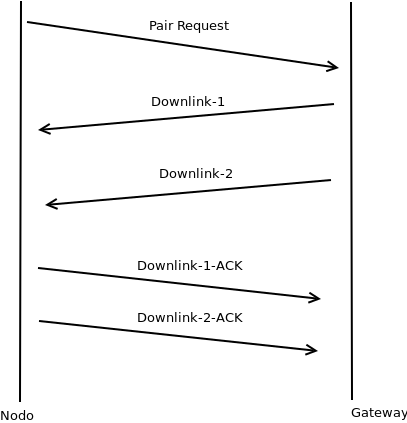
\includegraphics[scale=0.5]{diagramas/pair}
\caption{Diagrama de flujo de mensajes para fase de emparejamiento en red LoRa}
\label{pair:1}
\end{figure}
\newpage
\noindent
\clearpage
\subsection{Fase de Transmisión}

En el caso de que el nodo reciba bien ambos mensajes de bajada, como se observa en la Fig~\ref{trans:1}, se enviará un mensaje de petición de envío de datos (uplink request), a lo que en condiciones ideales (sin colisiones ni saturación de canal), el Gateway deberá responder con una confirmación de la petición de envío, deteniendo cualquier transmisión por aquel canal y quedando a la espera de la recepción del mensaje proveniente del nodo. El nodo una vez que recibe el paquete de confirmación de la petición de envío (ACK), este envía el paquete de datos al Gateway, donde en caso de no haber colisión, el Gateway respondería nuevamente con un paquete ACK, terminando con esto la fase de transmisión.\\


\begin{figure}[!ht]
\centering
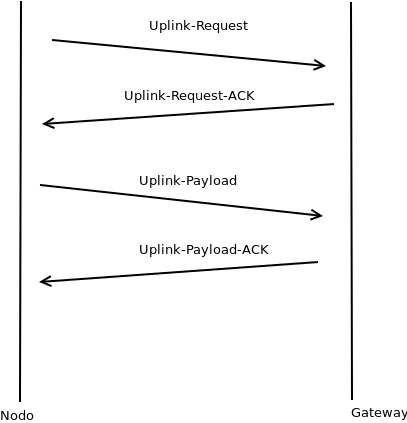
\includegraphics[scale=0.6]{diagramas/transmit}
\caption{Diagrama de flujo de mensajes en fase de transmisión de paquetes en red LoRa}
\label{trans:1}
\end{figure}
\newpage
\subsubsection{Fase de Retransmisión}
\justify
En el caso de que en cualquier fase ocurra una colisión o una interferencia que corrompa un bit en un paquete, el paquete será descartado y no llegará a destino, por lo que todos los dispositivos LoRa poseen un indicador de tiempo agotado (Timeout) el que es igual a:
 
\begin{eqnarray}
 Timeout(ms) = 2*(Time on Air)(ms)\end{eqnarray} \\
, donde \begin{eqnarray}
 Time on Air(ms)= \frac{Largo del Paquete}{Tx Data Rate}\end{eqnarray}
\noindent
En la Fig~\ref{retrans:1} se describe el proceso lógico que realiza el simulador en caso de no recibir un paquete ACK luego de la petición de conexión, en el caso que el tiempo transcurrido sea mayor al valor de la variable Timeout, el nodo volverá al estado previo de envío dependiendo si está pareado o no. En el caso de que se encuentre emparejado, volverá a la fase de transmisión para transmitir nuevamente el paquete uplink-request hasta que el Gateway le responda. Si el nodo no está emparejado, este volverá a la fase de emparejamiento donde enviará el paquete pair-request, hasta que el Gateway le responda con las dos ventanas de bajada (Downlink-1 y Downlink-2).
\begin{figure}[!ht]
\centering
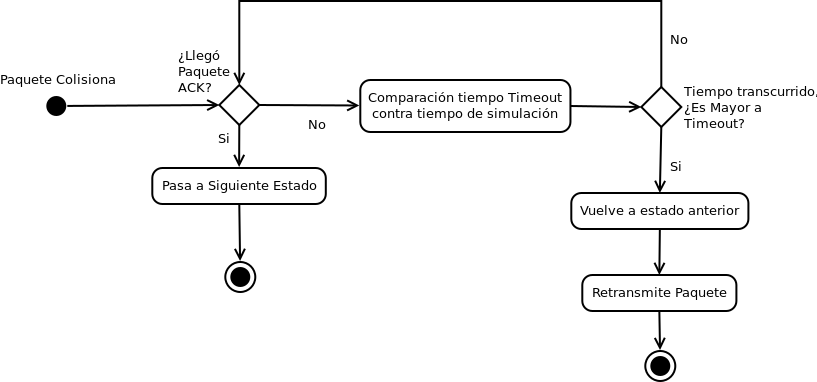
\includegraphics[scale=0.35]{diagramas/retrans}
\caption{Diagrama de estados que representa la fase de Retransmisión}
\label{retrans:1}
\end{figure}
\subsection{Fase de Reposo}
Luego de la transmisión del paquete uplink-payload desde el nodo al Gateway, si el Gateway contesta nuevamente con un último paquete de confirmación ACK, en este paquete el Gateway enviará los datos de su reloj interno para sincronizar y calendarizar el próximo envío de datos, a lo que el nodo sincroniza su reloj interno y entra en un estado de reposo, a lo que no transmite ni recibe nada hasta que se cumpla la condición entregada por el Gateway (tiempo de reposo es configurable desde los comando MAC del Gateway)
\subsection{Pérdida de Paquetes}
Con el fin de acercar mas a la realidad el modelo de simulación, se programó una función que simula la pérdida de paquetes en los distintos Spreading Factors, esto lo realiza llevando una contabilidad de los paquetes recibidos, y genera una comparativa con el porcentaje de pérdida de paquetes donde se tienen tres condiciones principales. La primera es que el porcentaje de pérdida de paquetes sea mayor que cero, y esta debe ser siempre verdadera, dado que si fuera cero no debería entrar a la función que desechará paquetes. La segunda condición es una condición compuesta, donde debe cumplirse que el coeficiente entre el contador de paquetes con error por el contador de paquetes recibidos (correctamente) multiplicado por cien, debe ser menor que el porcentaje de pérdida de paquetes, o en cambio es posible de que se cumpla de que el contador de errores sea igual a cero, con lo que también entraría a la función que desechará paquetes.\\
Con esta función es posible emular un ambiente más real al poder incluir condiciones desfavorables en la simulación, como las que son posibles de encontrar en la vida real.

%%%PRUEBAS%%%%
\section{Parámetros y Variables en Mediciones}
Para verificar el funcionamiento del modelo de simulación de los dispositivos LoRa, se establecieron ciertos parámetros a medir, los que serán a posterior indicadores del buen o mal funcionamiento del modelo de simulación. Estos parámetros son, los cambios de estado de los dispositivos LoRa (en el caso del simulador), para verificar que está realizando todo el proceso de forma correcta. Además, se medirá el número de colisiones contra la cantidad de mensajes enviados y erróneos, para calcular el porcentaje de pérdida de paquetes estimado en cada prueba de transmisión. Estas pruebas se realizarán primero en el ambiente real, con el fin de obtener un valor estimado del porcentaje de pérdida de paquetes real, el que luego se aplicará al modelo simulado y será contrastado tanto entre el ambiente real, el ambiente virtual, como también contra los porcentajes de pérdida de paquetes obtenido de \cite{Juha}.Este contraste de resultados, es realizado ya que el modelo de simulación, es desarrollado en un principio en una condición ideal de transmisión, por lo que no es afectado por ninguna variable del ambiente(interferencia por otras señales, edificios, interferencia por fuentes de poder,etc.) lo que lo hace poco real y por tanto no fiable como modelo de simulación, por lo que el objeto de este contraste es volver más fiable el modelo, agregando condiciones presentes en la realidad, al canal de transmisión virtual.\\
Adicionalmente para las pruebas de simulación se dispuso una distribución específica de los nodos para cada canal o Spreading Factor, dicha distribución es posible de encontrar en la Tab~\ref{tab:prueba}, donde se mostrará que cantidad de nodos está asignado a cada Spreading Factor, y que distancia en metros se le asignó para temas de la simulación. Estos datos explican la distribución de hasta diez nodos, la cual para las pruebas de cien nodos fue repetida diez veces con el fin de mantener la misma distribución pareja de nodos.Cabe decir que la correspondencia entre la distancia desde los nodos hasta el Gateway con el Spreading Factor asignado, fue tomado de datos de los desarrolladores en \cite{orange}.\\
En relación a las pruebas de cambio de estado, en la Tab~\ref{tab:estados} se muestran la correspondencia de cada valor numérico con cada estado de los nodos durante la simulación. Dentro de los estados disponibles para los nodos se encuentran los siguientes:
\begin{itemize}
\item IDLE: Este estado es el inicial para cada nodo en la red, es el encargado de enviar el pair request al Gateway y luego quedarse a la espera de recibir las dos ventanas de descarga desde el Gateway.
\item PRERECEIVE: Este estado sólo se encarga de esperar hasta que el Gateway envíe ambas ventanas de descarga, donde al llegar estas, y el nodo no estar emparejado, envía la orden de cambiara a estado TRANSMIT.
\item TRANSMIT: Este estado es activado al recibir las ventanas de descarga, es el estado que genera los mensajes Downlink-1-ack y Downlink-2-ack, los cuales serán enviados al Gateway para certificar de que se recibió la información de estos paquetes, los que en el caso de un emparejamiento real tendría relación con los identificadores de red, identificadores de aplicación y los tiempos que debe esperar entre cada ventana de subida de información.
\item RECEIVE: En este estado, se envía el primer ACK correspondiente a la primera ventana de descarga. Este estado da paso directo al estado RECEIVE2, dado que la diferencia de recepción de envío de la primera y segunda ventana, es poca en comparación con el resto de mensajes, esto permite la correcta recepción de ambos mensajes, sin pérdida del primero o falla de sincronización de la fase de emparejamiento por un sobre encolado de mensajes.
\item RECEIVE2 : En este estado, se envía el segundo paquete ACK correspondiente a la segunda ventana de descarga. Este estado da paso directo al estado al estado IDLE2 , con el fin de cumplir la ventana de tiempo antes de enviar información hacia el Gateway y no colisionar con otro envío de información.
\item IDLE2: Este estado es el encargado de enviar la petición de subida de información al Gateway, con el fin de evitar pérdida de datos de medición en caso de que el Gateway no esté disponible para el recibimiento de esta información. Este estado da el paso al estado ACK, para poder recibir el primer ACK correspondiente a esta petición.
\item ACK: En esta estado se activa sólo si es recibido el ACK correspondiente a la petición de envío de información y si el estado anterior fue IDLE2. Si es recibido este ACK, el nodo envía el payload correspondiente a la información de medición que posee en ese instante al Gateway y queda a la espera de el paquete ack-payload-2. Este estado da paso al estado SLEEP.
\item ACK2: Este estado fue creado con el fin de depurar la interacción entre Gateway y nodos, por lo que para las pruebas y el uso actual del simulador, no posee uso funcional.
\item SLEEP: Este estado se activa luego de recibir el paquete ack-payload-2 correspondiente a el Payload enviado desde el nodo al Gateway, donde luego se colocará al nodo en estado de reposo hasta la siguiente ventana de envío. Una vez cumplido el tiempo de espera del nodo, este volverá al estado IDLE2 para volver al ciclo de envío de datos. Luego de este estado, no se vuelve al estado de emparejamiento, dado que sólo es necesario emparejar una vez con el Gateway de la red, a menos que se posea una topología estrella-estrella que requiera otro tipo de interacción, el cual no es abarcado por este proyecto.
\end{itemize}

\begin{table}[!ht]
\centering
\begin{tabular}{|c|c|c|}
\hline
Número de Host & Spreading Factor & Distancia a Gateway [Metros]\\ 
\hline
1 & 7 & 1 \\
\hline
2 & 7 & 2 \\
\hline
3 & 8 & 3 \\
\hline
4 & 8 & 4 \\
\hline
5 & 9 & 5 \\
\hline
6 & 9 & 6 \\
\hline
7 & 10 & 7 \\
\hline
8 & 11 & 11 \\
\hline
9 & 12 & 14 \\
\hline
10 & 12 & 14 \\
\hline
\end{tabular}
\caption{Tabla con distribución de nodos en cada Spreading Factor para pruebas de simulación}
\label{tab:prueba}
\end{table}

\begin{table}[!ht]
\centering
\begin{tabular}{|c|c|c|}
\hline
Indicador de estado & Estado de nodo\\ 
\hline
0& IDLE \\
\hline
1& TRANSMIT \\
\hline
2& PRERECEIVE\\
\hline
3& RECEIVE\\
\hline
4& RECEIVE2\\
\hline
5& IDLE2\\
\hline
6& ACK\\
\hline
7& ACK2\\
\hline
8& SLEEP\\
\hline

\end{tabular}
\caption{Tabla con relación de indicador de estado y estado alcanzado por cada nodo en la simulación}
\label{tab:estados}
\end{table}

\subsection{Pruebas Realizadas}
Las pruebas realizadas constan de dos tipos, la que comprueba los cambios de estado de los nodos para verificar el correcto funcionamiento de la lógica de los dispositivos LoRa aplicados en el modelo de simulación dependiendo de la cantidad de nodos, y para verificar la demora del emparejamiento en casos de mayor saturación del canal, y las prueba de transmisión donde tanto los dispositivos reales como los virtuales, tendrán las mismas configuraciones iniciales, y donde se obtendrá el porcentaje de pérdida de paquetes, dato con el que se podrá establecer que porcentaje de sensibilidad posee el modelo de simulación y con esto validarlo, o establecer un ajuste, para alcanzar el nivel de sensibilidad esperado. Asimismo se generaron pruebas de transmisión en el simulador con 1, 10 y 100 nodos, con el fin de determinar el crecimiento del número de colisiones que generan por canal (Spreading Factor) los nodos, y de la misma forma para determinar la sensibilidad alcanzada en la simulación de pérdidas de paquetes agregada al modelo de simulación.

\section{Resultados Obtenidos}
\subsection{Cambios de Estado}
Se realizaron dos instancias de esta prueba, la primera con un número menor a la cantidad de Spreading Factor disponibles, con el fin de corroborar la correcta transición de estados en una transmisión ideal, es decir, sin colisiones ni pérdidas de paquetes (Véase Fig~\ref{prueba:1}).La segunda instancia se realizó con cincuenta nodos, con el fin de ver como responde frente a las colisiones y retransmisiones(Véase Fig~\ref{prueba:2} y Fig~\ref{prueba:3}).
\begin{figure}[!ht]
\centering
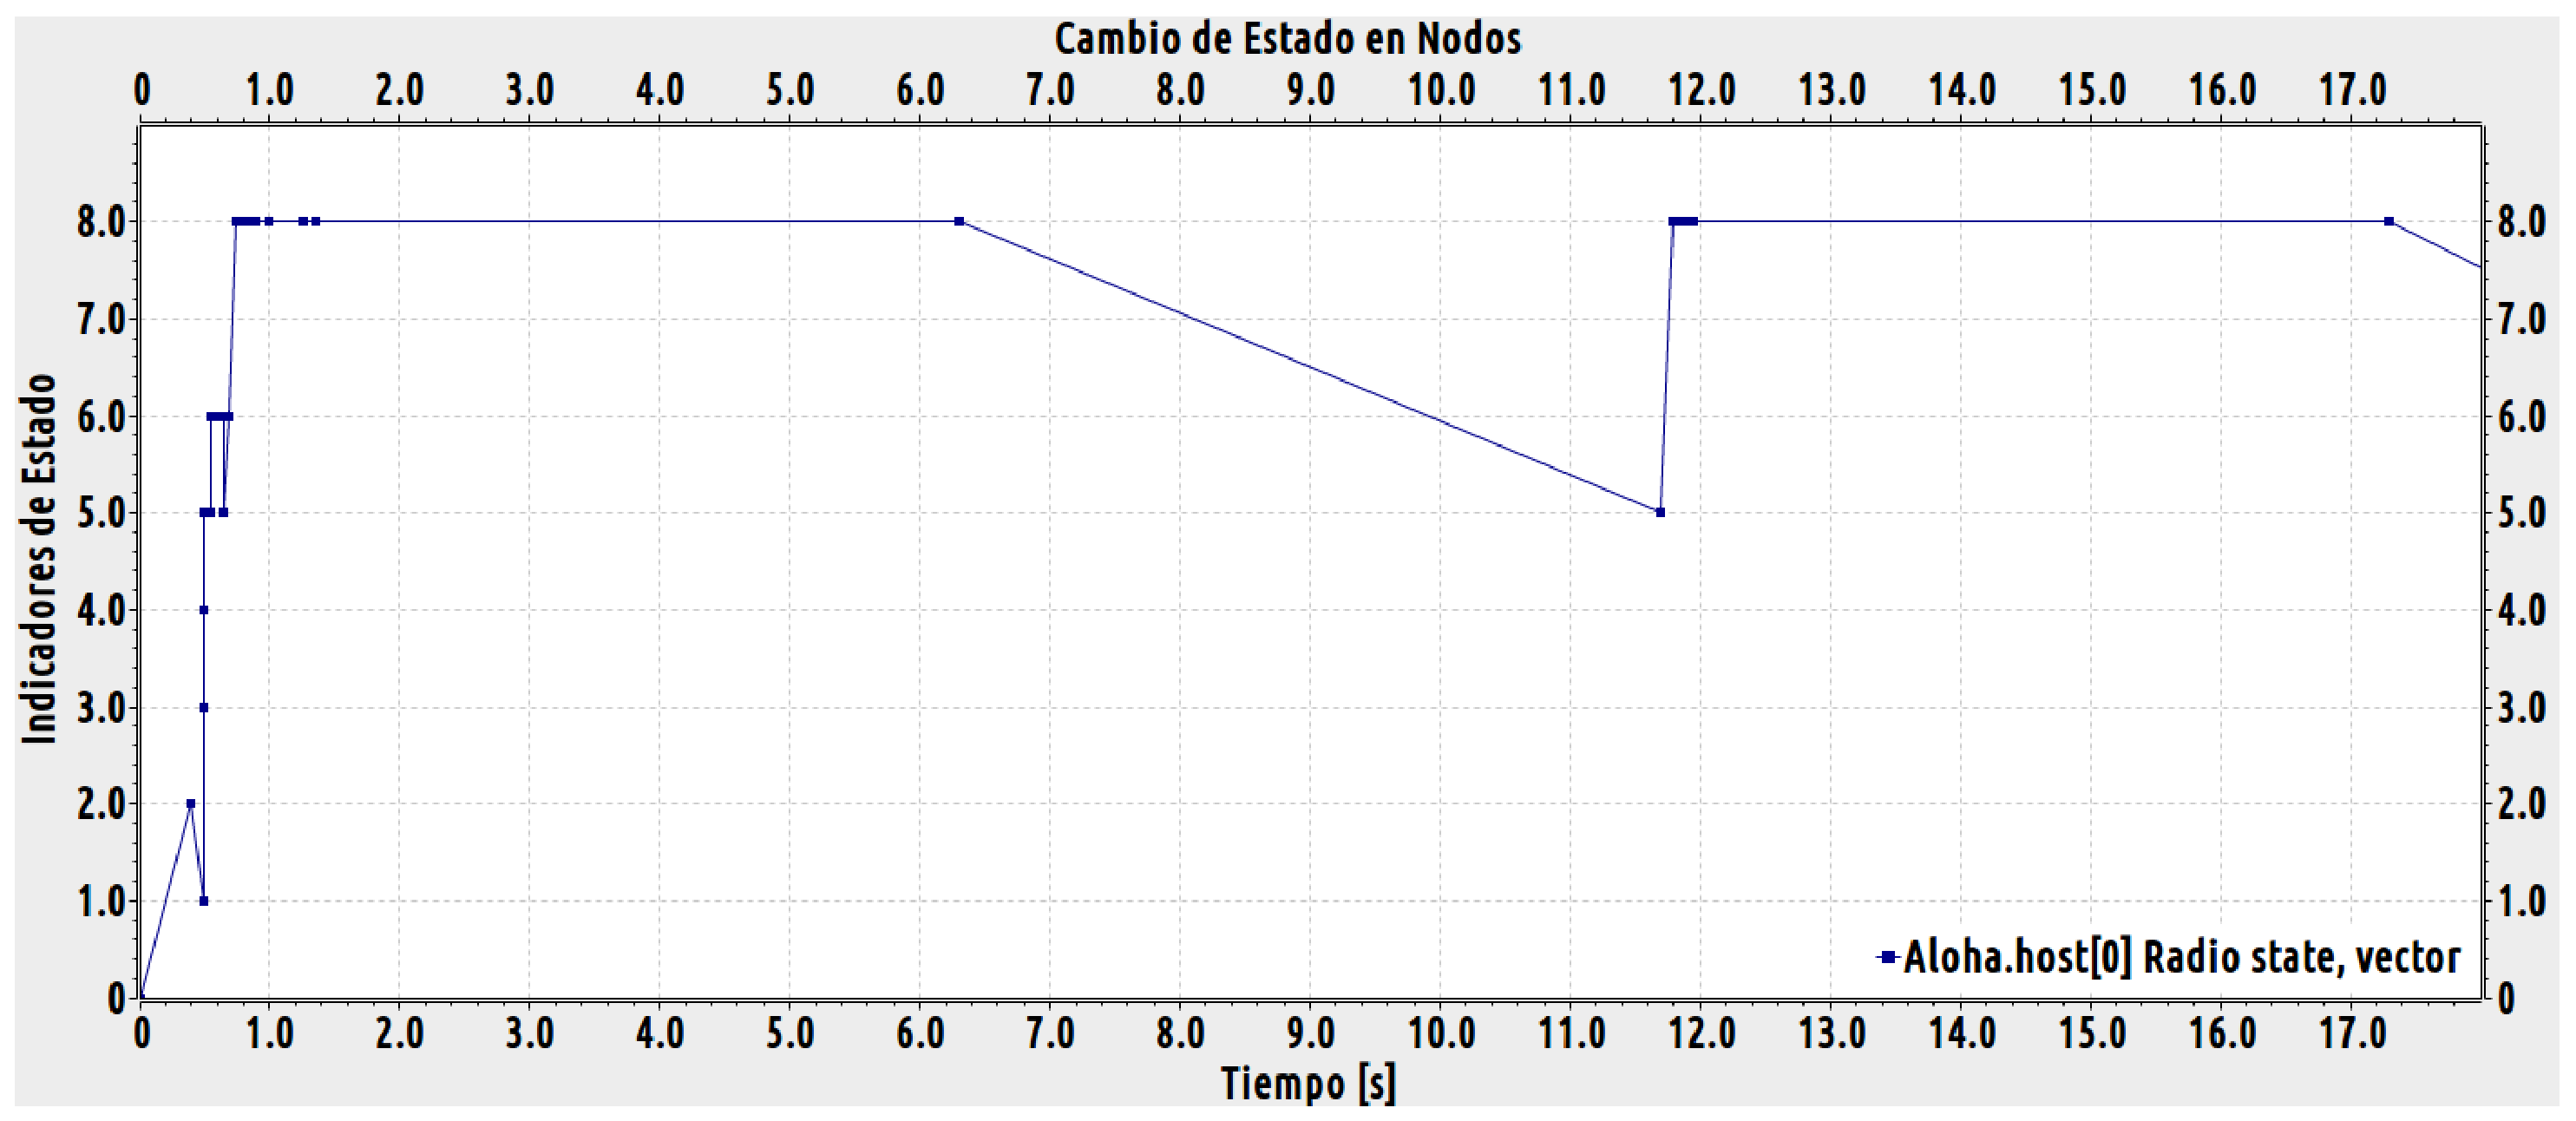
\includegraphics[width=13cm,height=30cm,keepaspectratio]{images/cambioestado1nodo-ideal.eps}
\caption{Cambios de estados por tiempo en segundos , con un nodos transmitiendo.\textit{Esta imagen \\
puede verse ampliada en el Anexo~\ref{anexa:1}}}
\label{prueba:1}
\end{figure}
En la Fig~\ref{prueba:2} se encuentra un gráfico de cambios de estado según el tiempo transcurrido, pero esta vez con 10 nodos, con el fin de determinar cuanto demoran los nodos en realizar el proceso de emparejamiento con más nodos por canal.
%% pruebas con 10 nodos
\begin{figure}[!ht]
\centering
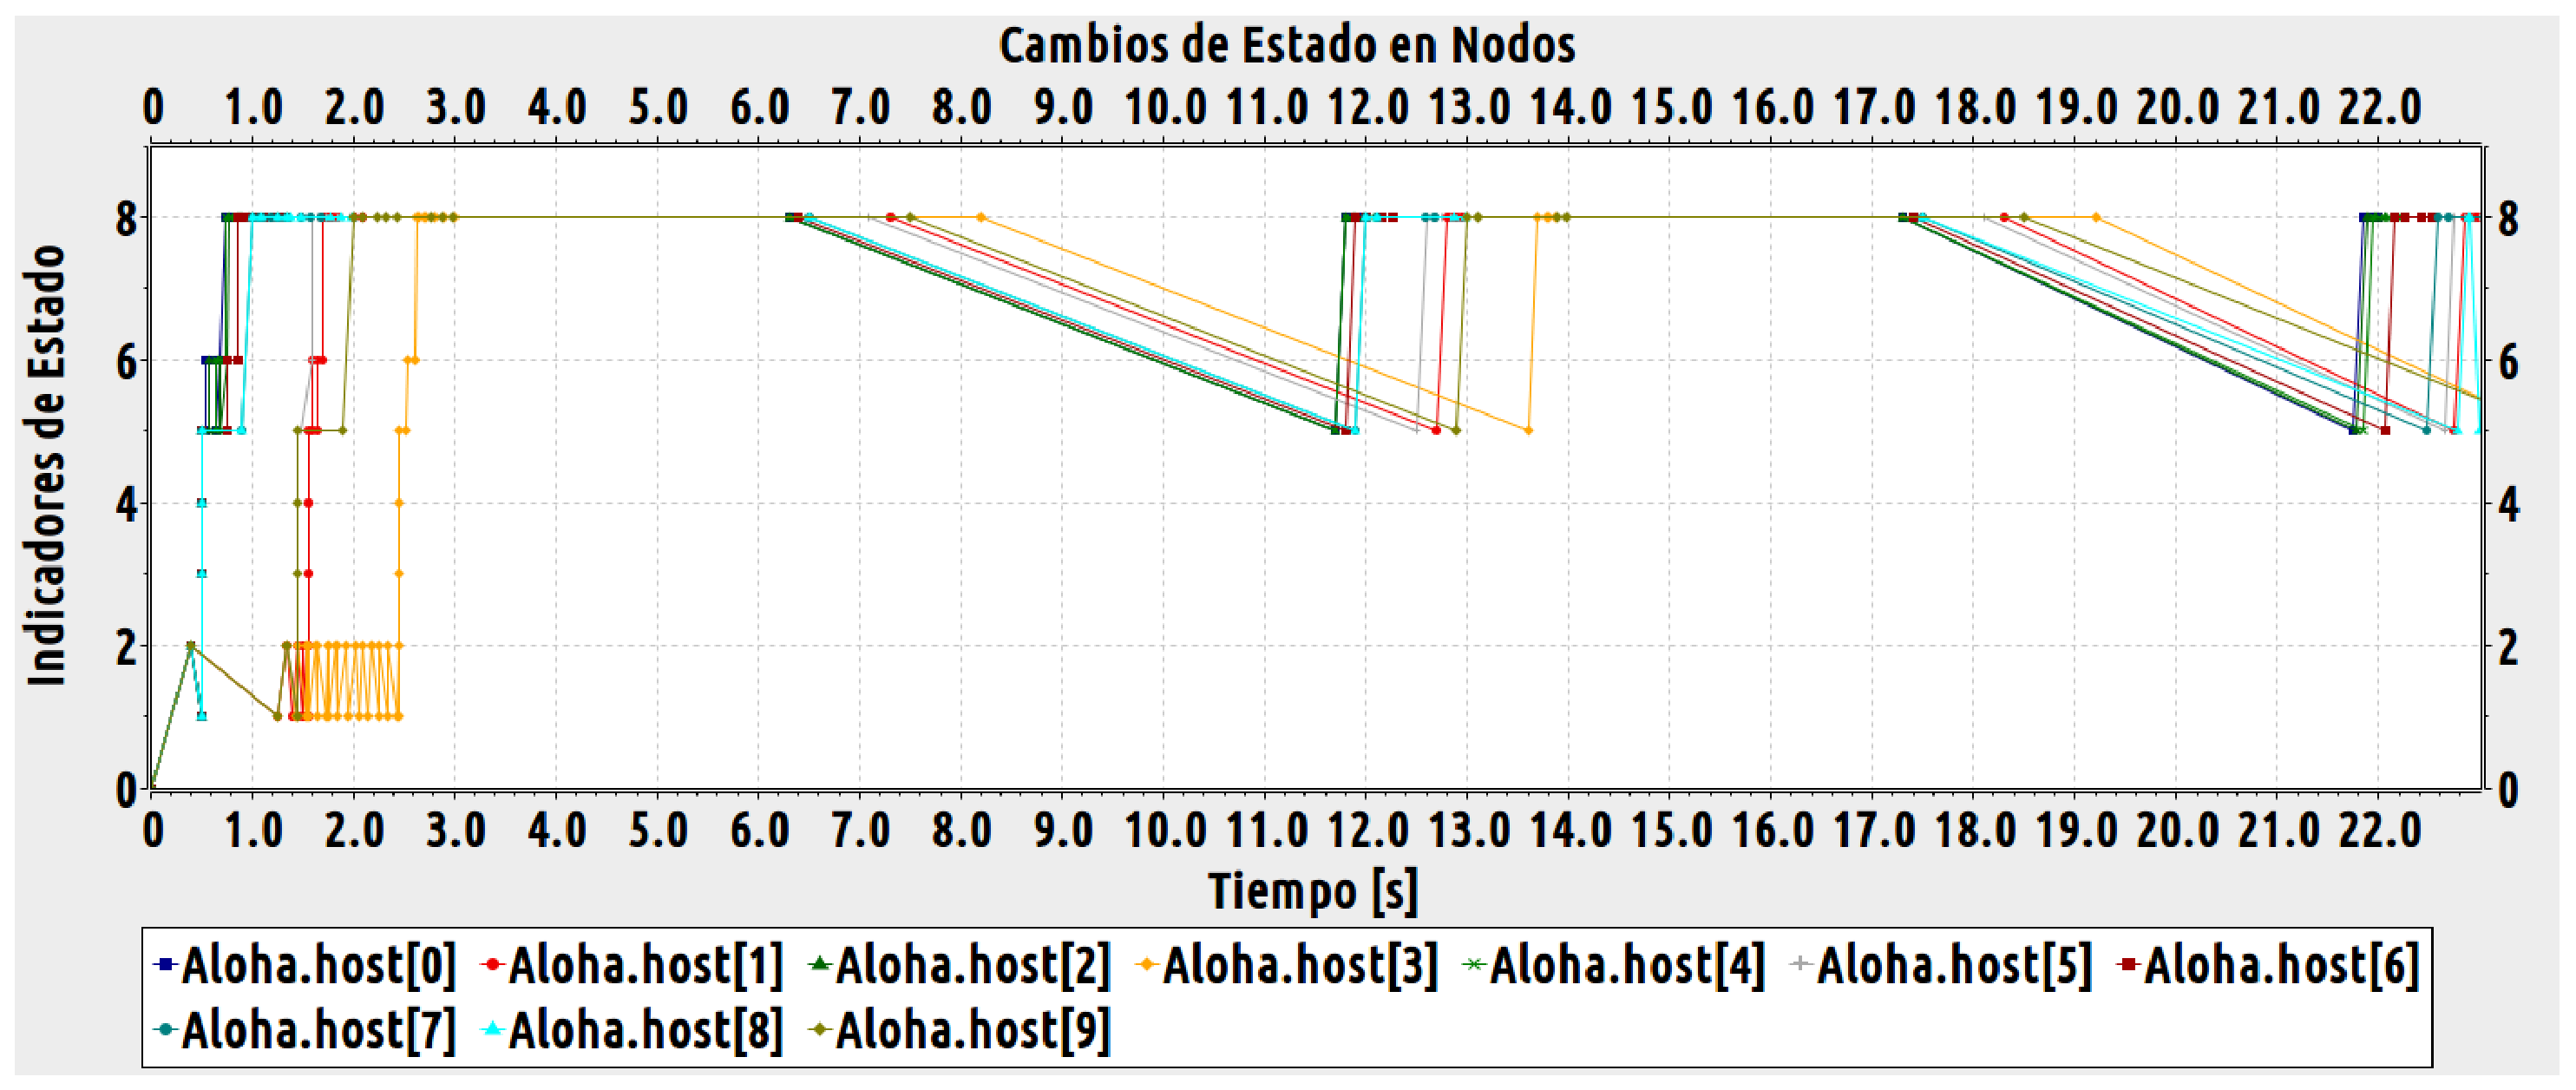
\includegraphics[width=13cm,height=30cm,keepaspectratio]{images/cambioestado10nodos.eps}
\caption{Gráfico de Cambios de estados por tiempo en segundos , con diez nodos transmitiendo.\textit{Esta imagen puede verse ampliada en el Anexo~\ref{anexa:2}}}
\label{prueba:2}
\end{figure}
En la Fig~\ref{prueba:3} se presenta un gráfico de cambios de estado donde esta vez se encuentran 100 nodos distribuidos de forma uniforme en los distintos canales disponibles. \\
En estos gráfico se aprecia de que a medida de que aumenta la cantidad de nodos, el proceso de emparejamiento se ve ralentizado dado que las colisiones dentro del canal comienzan a generar retransmisiones, las que poco a poco permiten el emparejamiento del total de nodos de la red, y dando inicio al ciclo de transmisión de datos (de medición, u otro tipo) desde los nodos al Gateway, para luego volver al estado de reposo hasta la próxima ventana de envío.\\
\begin{figure}[!ht]
\centering
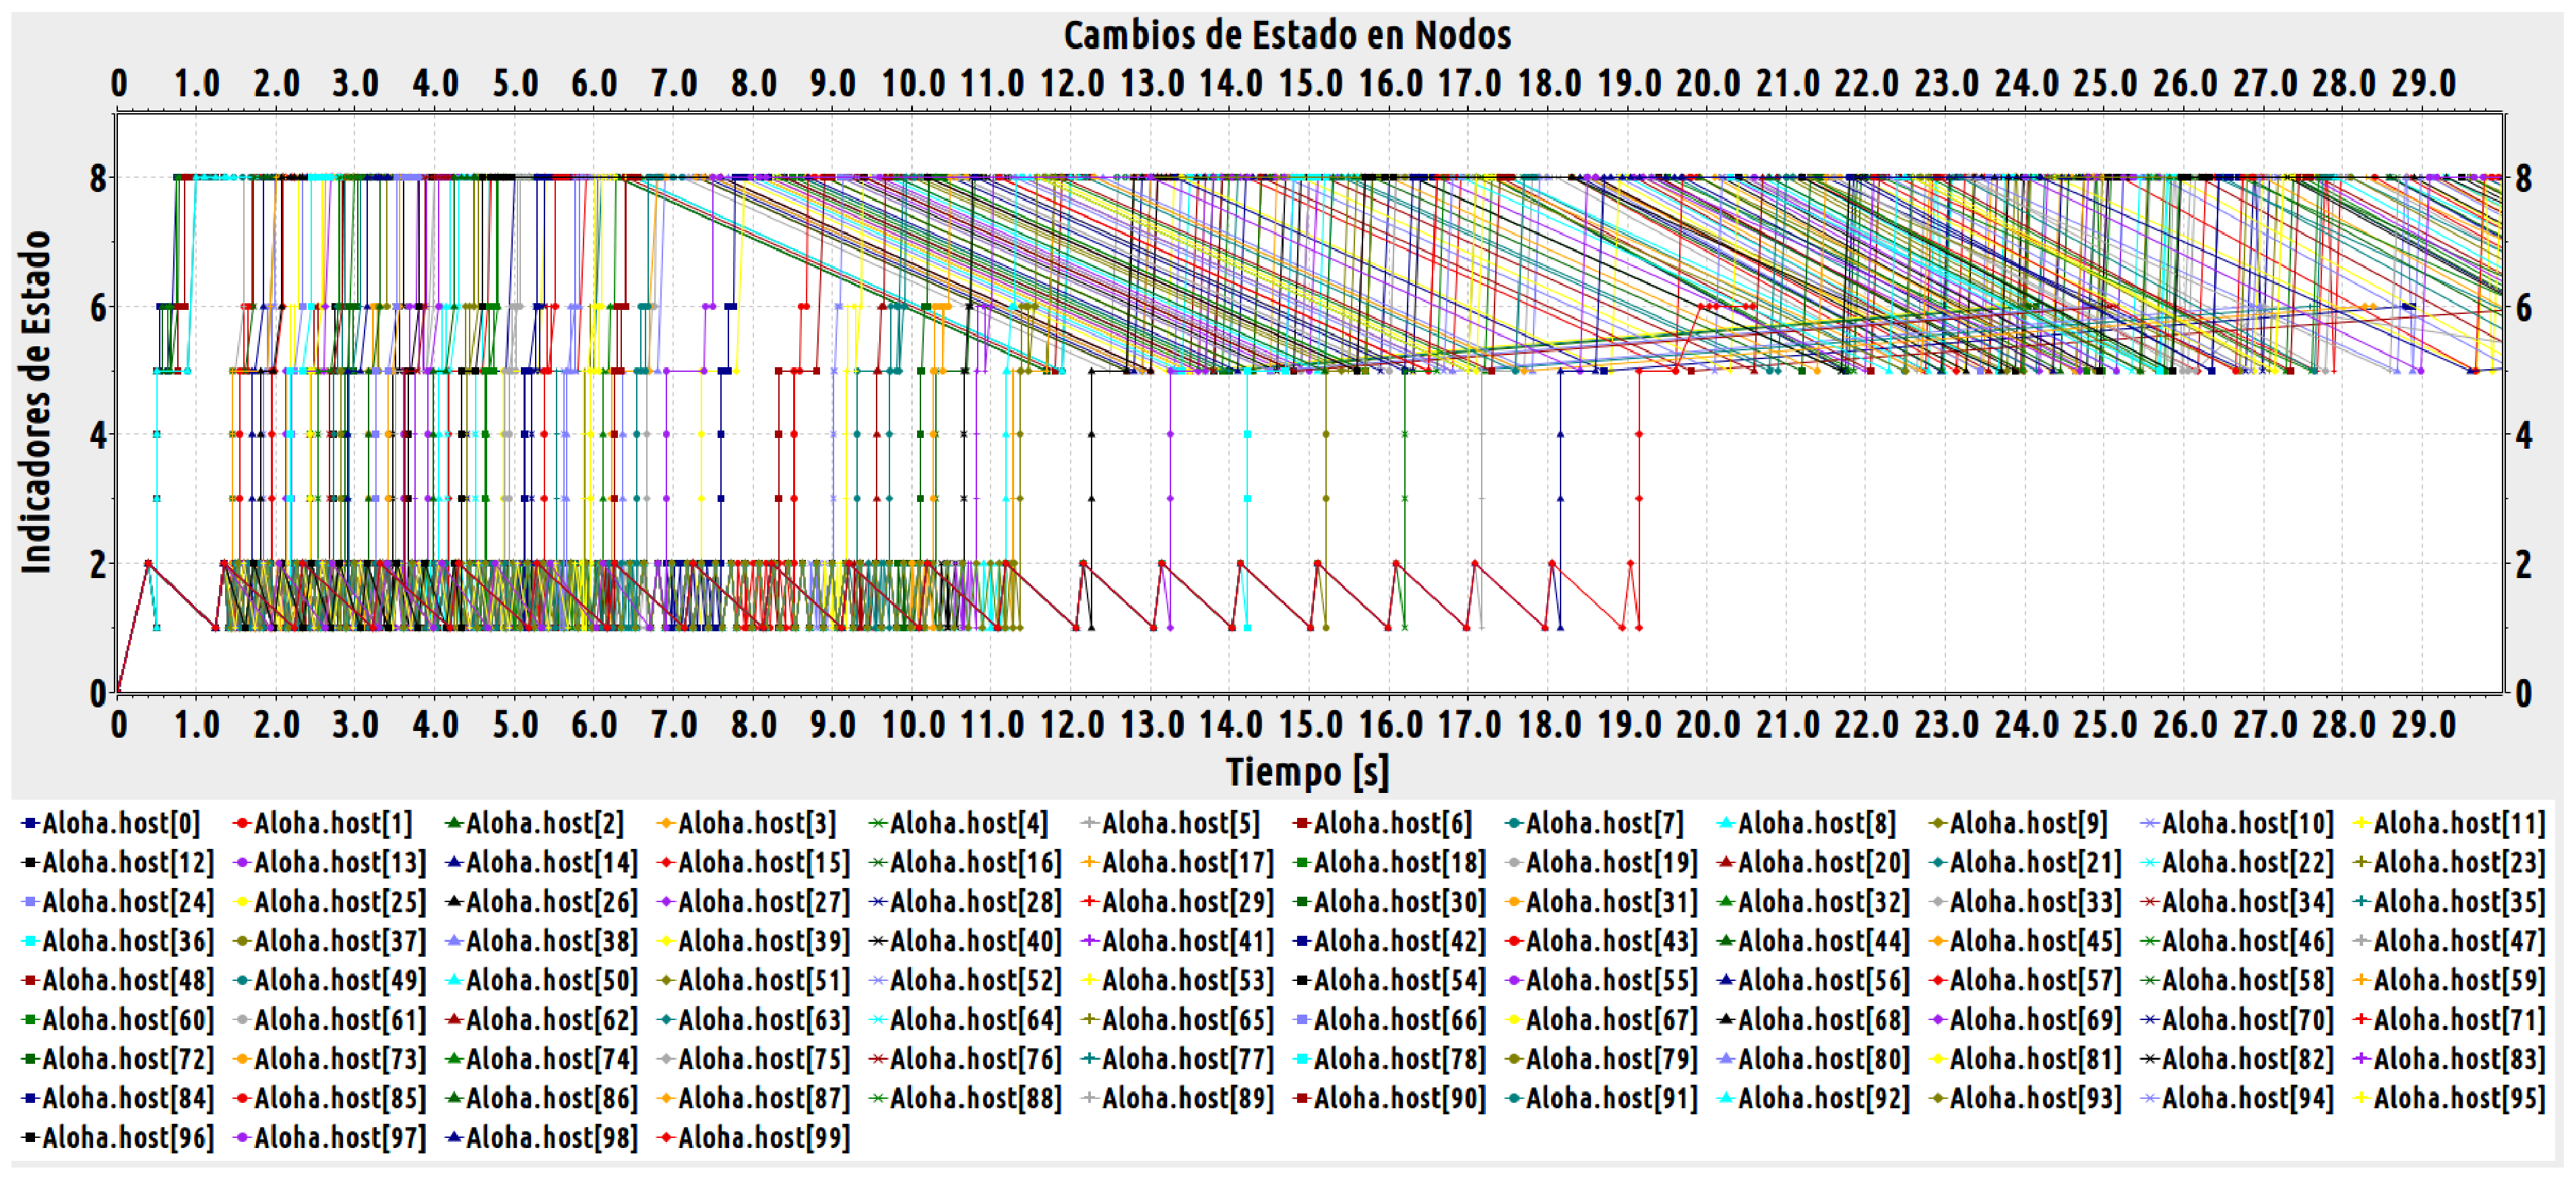
\includegraphics[width=13cm,height=30cm,keepaspectratio]{images/cambioestado100nodos.eps}
\caption{Gráfico de Cambios de estados por tiempo en segundos , con cien nodos transmitiendo.\textit{Esta imagen puede verse ampliada en el Anexo~\ref{anexa:3}}}
\label{prueba:3}
\end{figure}
\subsection{Pruebas de Transmisión en ambiente virtual}
En estas pruebas, se realizaron transmisiones de datos entre diez y cien nodos durante $42s$ de simulación, con el fin de detectar la cantidad de colisiones generadas por el aumento de la saturación de los canales utilizados. A través de estas mediciones se espera visualizar el nivel exponencial de retardo en el inicio de las distintas fases de los nodos por efecto de las colisiones y retransmisiones inherentes de comunicaciones basadas en el protocolo ALOHA. Cabe decir de que sólo existen colisiones dentro de cada Spreading Factor o canal, ya que entre los distintos Spreading Factors según las especificaciones técnicas de \cite{Sornin} y según las pruebas empíricas realizadas por \cite{Xavier}, se indica de que al usar la técnica de modulación de espectro expandido, basta con conocer la frecuencia base del mensaje para poder recibirlo y demodularlo sin problemas, dado que cualquier interferencia en el resto del espectro de la señal, será eliminado al momento de filtrar la señal con un filtro pasa banda, pasa bajo, etc., dependiendo del necesario para cada canal.\\
En la Fig~\ref{nodos:10}, se observa la cantidad de colisiones por cada Spreading Factor, donde la utilización de cada canal sería aproximadamente de 2 nodos por canal, lo que eventualmente es una saturación muy baja, lo que se traduce en un retardo pequeño en tiempo de el correcto inicio y finalización de los estados correspondientes a cada fase de la comunicación en los dispositivos LoRa.

\begin{figure}[!ht]
\centering
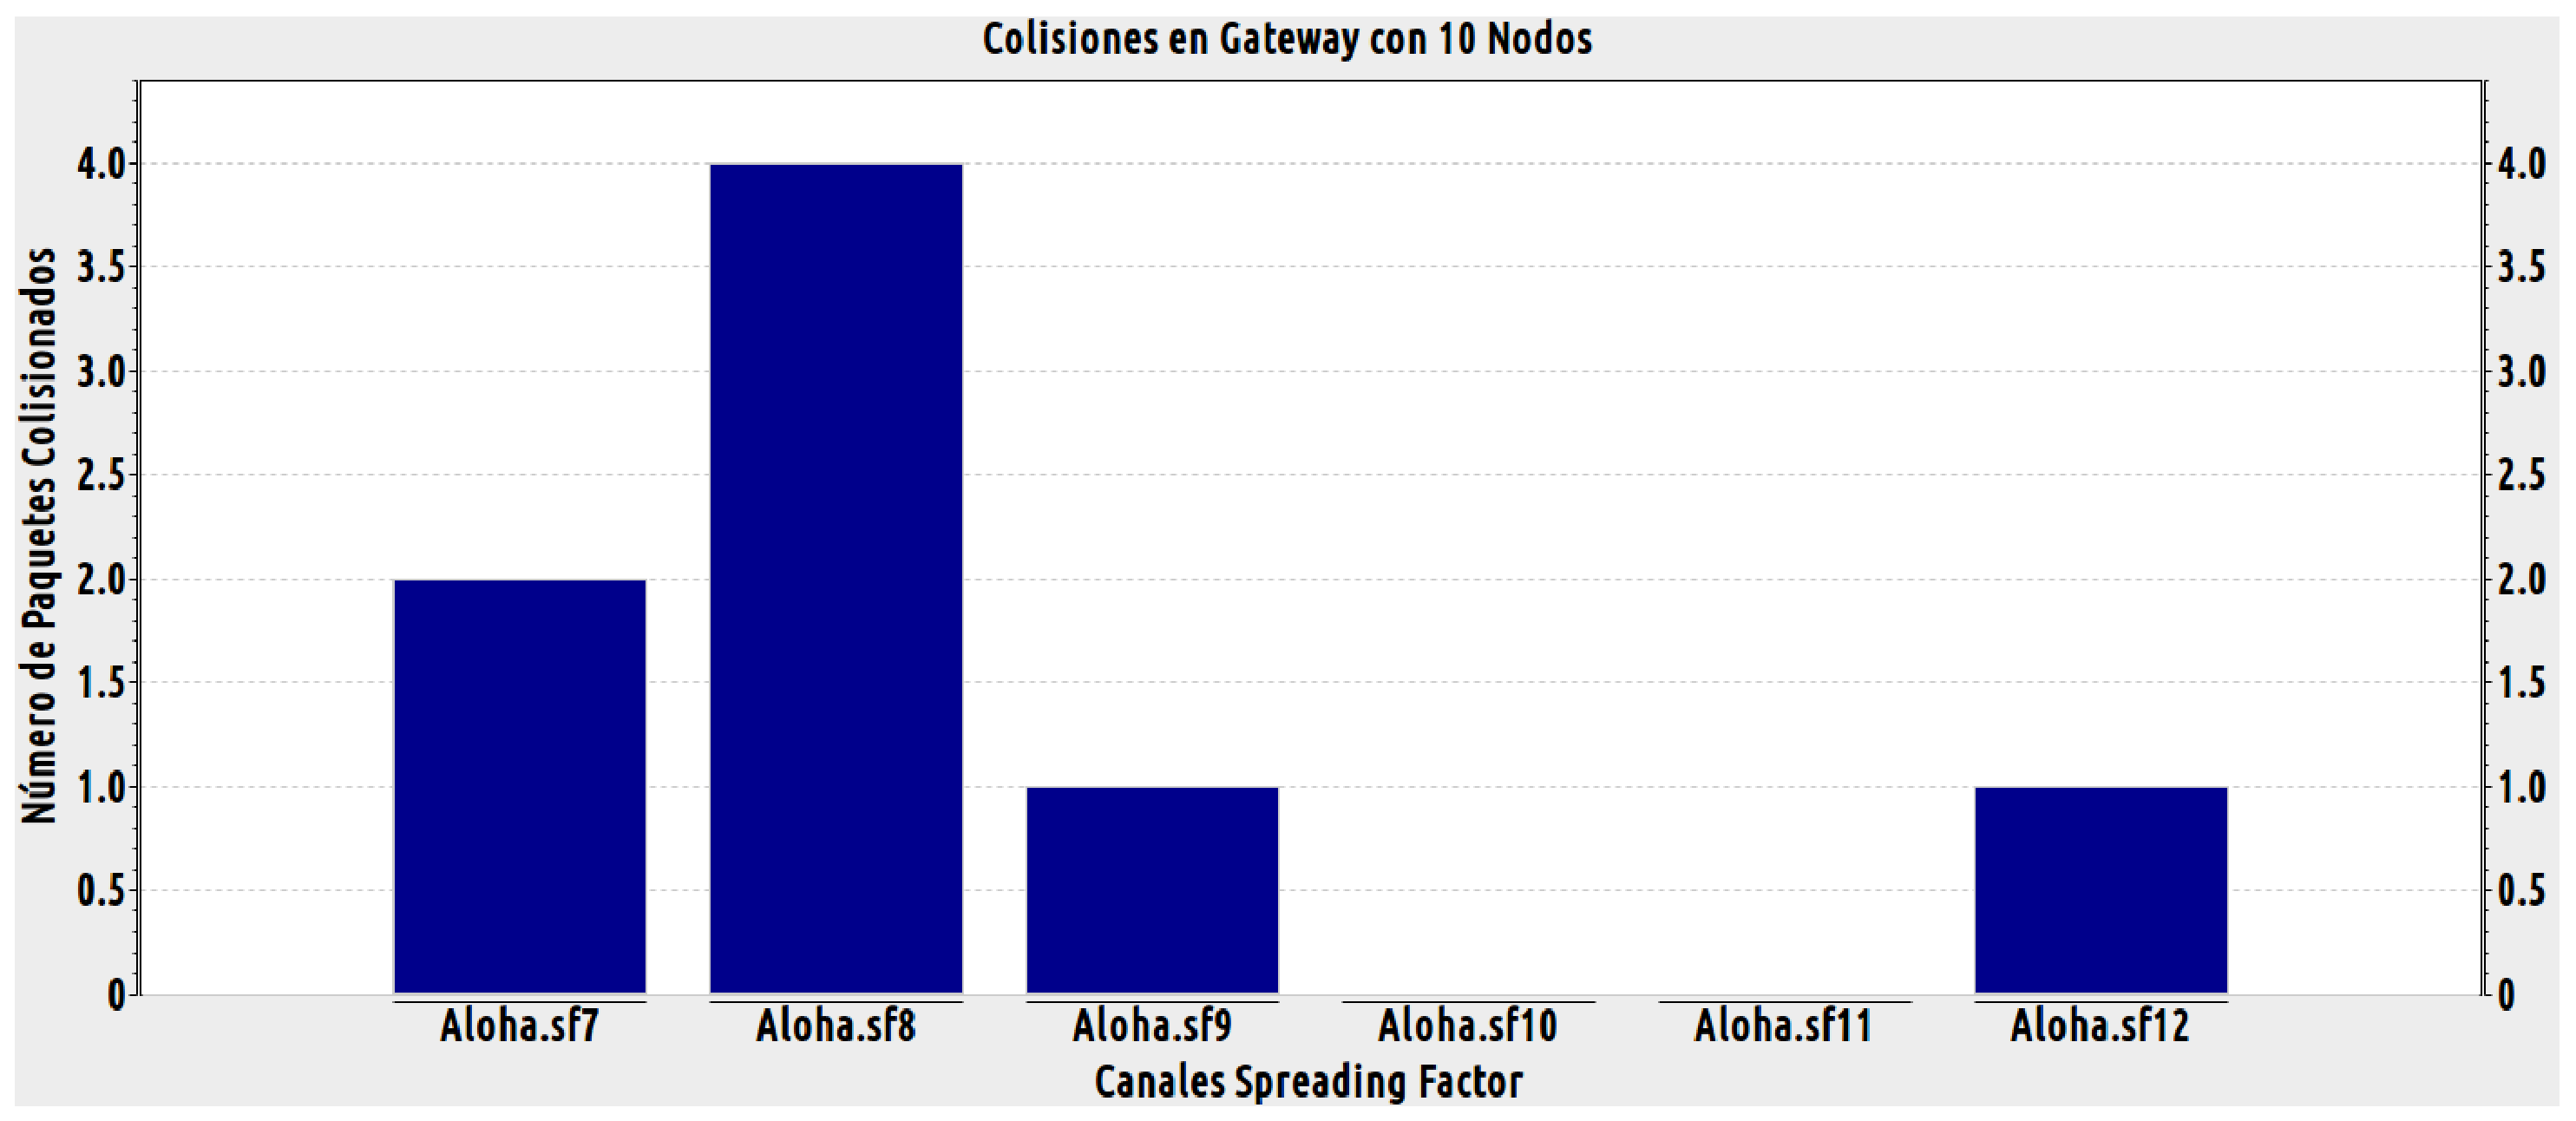
\includegraphics[width=13cm,height=30cm,keepaspectratio]{images/colisiones10nodos.eps}
\caption{Gráfico de colisiones ocurridos entre los distintos Spreading Factor, para 10 nodos transmitiendo.\textit{Esta imagen puede verse ampliada en el Anexo~\ref{anexb:1}}}
\label{nodos:10}
\end{figure}

En la Fig~\ref{nodos:100}, se contempla de que se sigue la misma distribución de colisiones, con la diferencia de que al aumentar los nodos, y la saturación del canal en diez veces a la prueba anterior, las colisiones suben en número también diez veces aproximadamente, excepto en el Spreading Factor 8, donde ocurre una anomalía en el comportamiento del modelo de simulación. El cual es explicado por el orden pseudo-aleatorio que posee el framework a la hora de indicar que nodo es el siguiente en enviar datos, esto conlleva a que sólo este Spreading Factor, posea este comportamiento fuera de lo normal (como el resto de los Spreading Factors). Esto también se explica, en que la simulación fue tomada por sólo $42s$ de simulación, por lo que los gráficos muestran el estado de la simulación en ese momento dado, sin embargo, es posible de que si se hubiera permitido seguir el tiempo de la simulación una cantidad de segundos más se podría apreciar un emparejamiento del número de colisiones obtenidas en todos los Spreading Factors. Este último efecto también ocurre al agregar un porcentaje de paquetes perdidos, dado que son índices que dependen mucho de en que fase se encuentren en ese segundo y que evento están queriendo representar. Para este caso en particular, no es importante el hecho de esta anormalidad, dado que se logra explicar el porqué del evento, junto con poder analizar el crecimiento del número de colisiones a mayor número de nodos.
\begin{figure}[!ht]
\centering
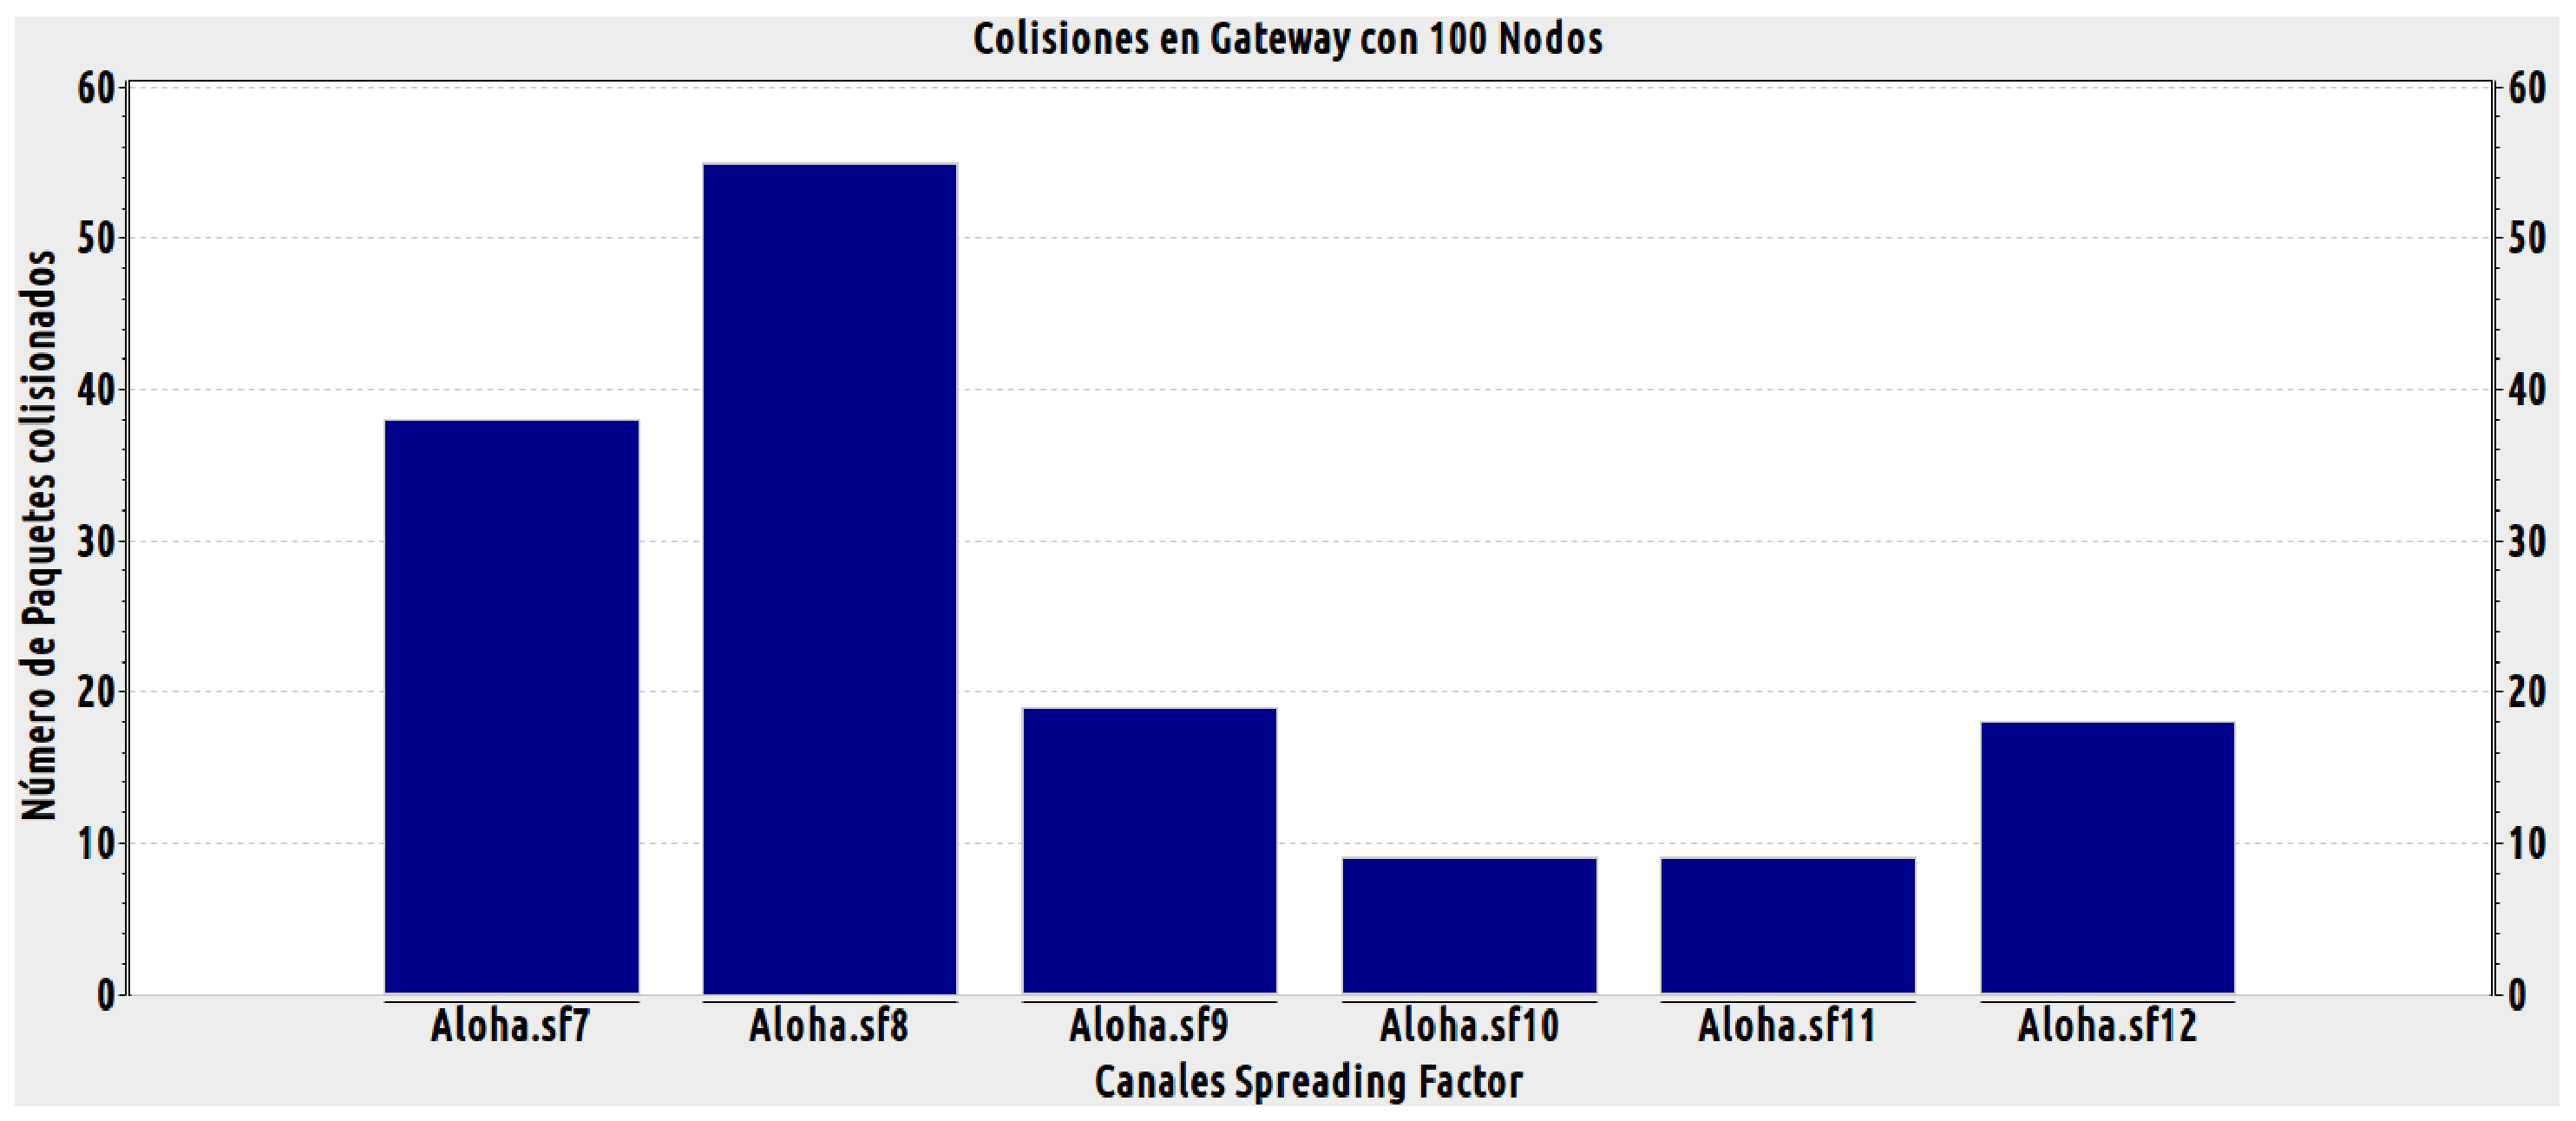
\includegraphics[width=13cm,height=30cm,keepaspectratio]{images/colisiones100nodos.eps}
\caption{Gráfico de colisiones ocurridos entre los distintos Spreading Factor, para 100 nodos transmitiendo.\textit{Esta imagen puede verse ampliada en el Anexo~\ref{anexb:2}}}
\label{nodos:100}
\end{figure}
\subsection{Pruebas de Transmisión en ambiente real}
%%pruebas dispositivos reales
%%en spreding factors
La prueba de transmisión, se realizó cinco veces para cada Spreading Factor para determinar el porcentaje de pérdida de paquetes en cada espectro de frecuencia y agregarlo al modelo de simulación. Para esta prueba se enviaron en promedio noventa y siete paquetes de datos, de los cuales sólo se recibió alrededor de treinta y siete paquetes en promedio, lo que corresponde a un $38\%$ de recepción de paquetes. La configuración usada para esta prueba corresponden a los valores definidos como constantes (Véase Tab~\ref{par:1}). A continuación se presentan los resultados (Véase Tab~\ref{prueba:3})
\begin{table}[!ht]
\centering
\begin{tabular}{|c|c|c|c|}
\hline
Spreading Factor & Paquetes Enviados & Paquetes Recibidos & Packet Loss \% \\ 
\hline
SF12 & 84 & 30 & 65,1\% \\
\hline
SF11 & 99 & 15 & 84,8\% \\
\hline
SF10 & 158 & 19 & 87.9\% \\
\hline
SF9 & 360 & 78 & 78.3\% \\
\hline
SF8 & 469 & 38 & 91.9\% \\
\hline
SF7 & 983 & 47 & 95.2\% \\
\hline
\end{tabular}
\caption{Tabla con resultados de pruebas de conectividad por Spreading Factor}
\label{prueba:3}
\end{table}

\subsection{Índice de Pérdida de Paquetes}
En relación a las pruebas de transmisión realizadas con los dispositivos físicos, se alejan mucho de los resultados esperados, e incluso de los datos que otorga la especificación de LoRa. Esto es causado por interferencia generada por la fuente de poder administrada a los dispositivos y una incorrecta forma de aislamiento de los conectores y partes conductoras de la placa, como también es posible que sea debido producto de la baja sensibilidad de la antena del Gateway, ya que todas las pruebas realizadas por investigadores como \cite{Xavier} y \cite{Juha}, donde los resultados que arrojan sus pruebas son muy satisfactorias, los Gateway están ubicados a una altura muy elevada (normalmente en torres fijas sobre los $20m$ de altura), y equipados con antenas bi-cónicas de alta sensibilidad, lo que permite una transmisión a mucha más distancia que el mismo Gateway con una antena de sensibilidad más modesta.\\
De acuerdo a este contexto, se decidió adoptar el porcentaje de pérdida de paquetes que entregan las distintas mediciones realizadas por otros investigadores ($PacketLoss[\%]=1\%$), se asemejan más a la norma y a las especificaciones de ~\cite{Xavier} y de~\cite{Juha}.

\subsection{Resultados Obtenidos agregando Pérdida de Paquetes}
Dentro de las pruebas de transmisión en el ambiente virtual, también se registró la cantidad de paquetes con errores (que no llegaron a destino), los que en un ambiente real pueden tener el carácter de interferencia. Para el modelo de simulación el porcentaje de pérdida de paquetes, se mide en cada transmisión en base al PER ingresado, junto a la cantidad de paquetes recibidos por cada Spreading Factor, por lo que dependiendo de que Spreading Factor posea más envíos efectivos de mensajes (en el caso de que uno haya entrado antes al estado de transmisión que otro nodo).\\
Como es posible notar en la Fig~\ref{prueba:4}, la cantidad de paquetes con errores es similar en todos los Spreading Factor (con un PER del 1\%), por lo que al menos con diez nodos, la función que calcula la pérdida de paquetes y la hace efectiva, dependiendo del número de paquetes recibidos, es efectiva en un nivel bajo de saturación de canal.
%%pruebas con 5 nodos
\begin{figure}[!ht]
\centering
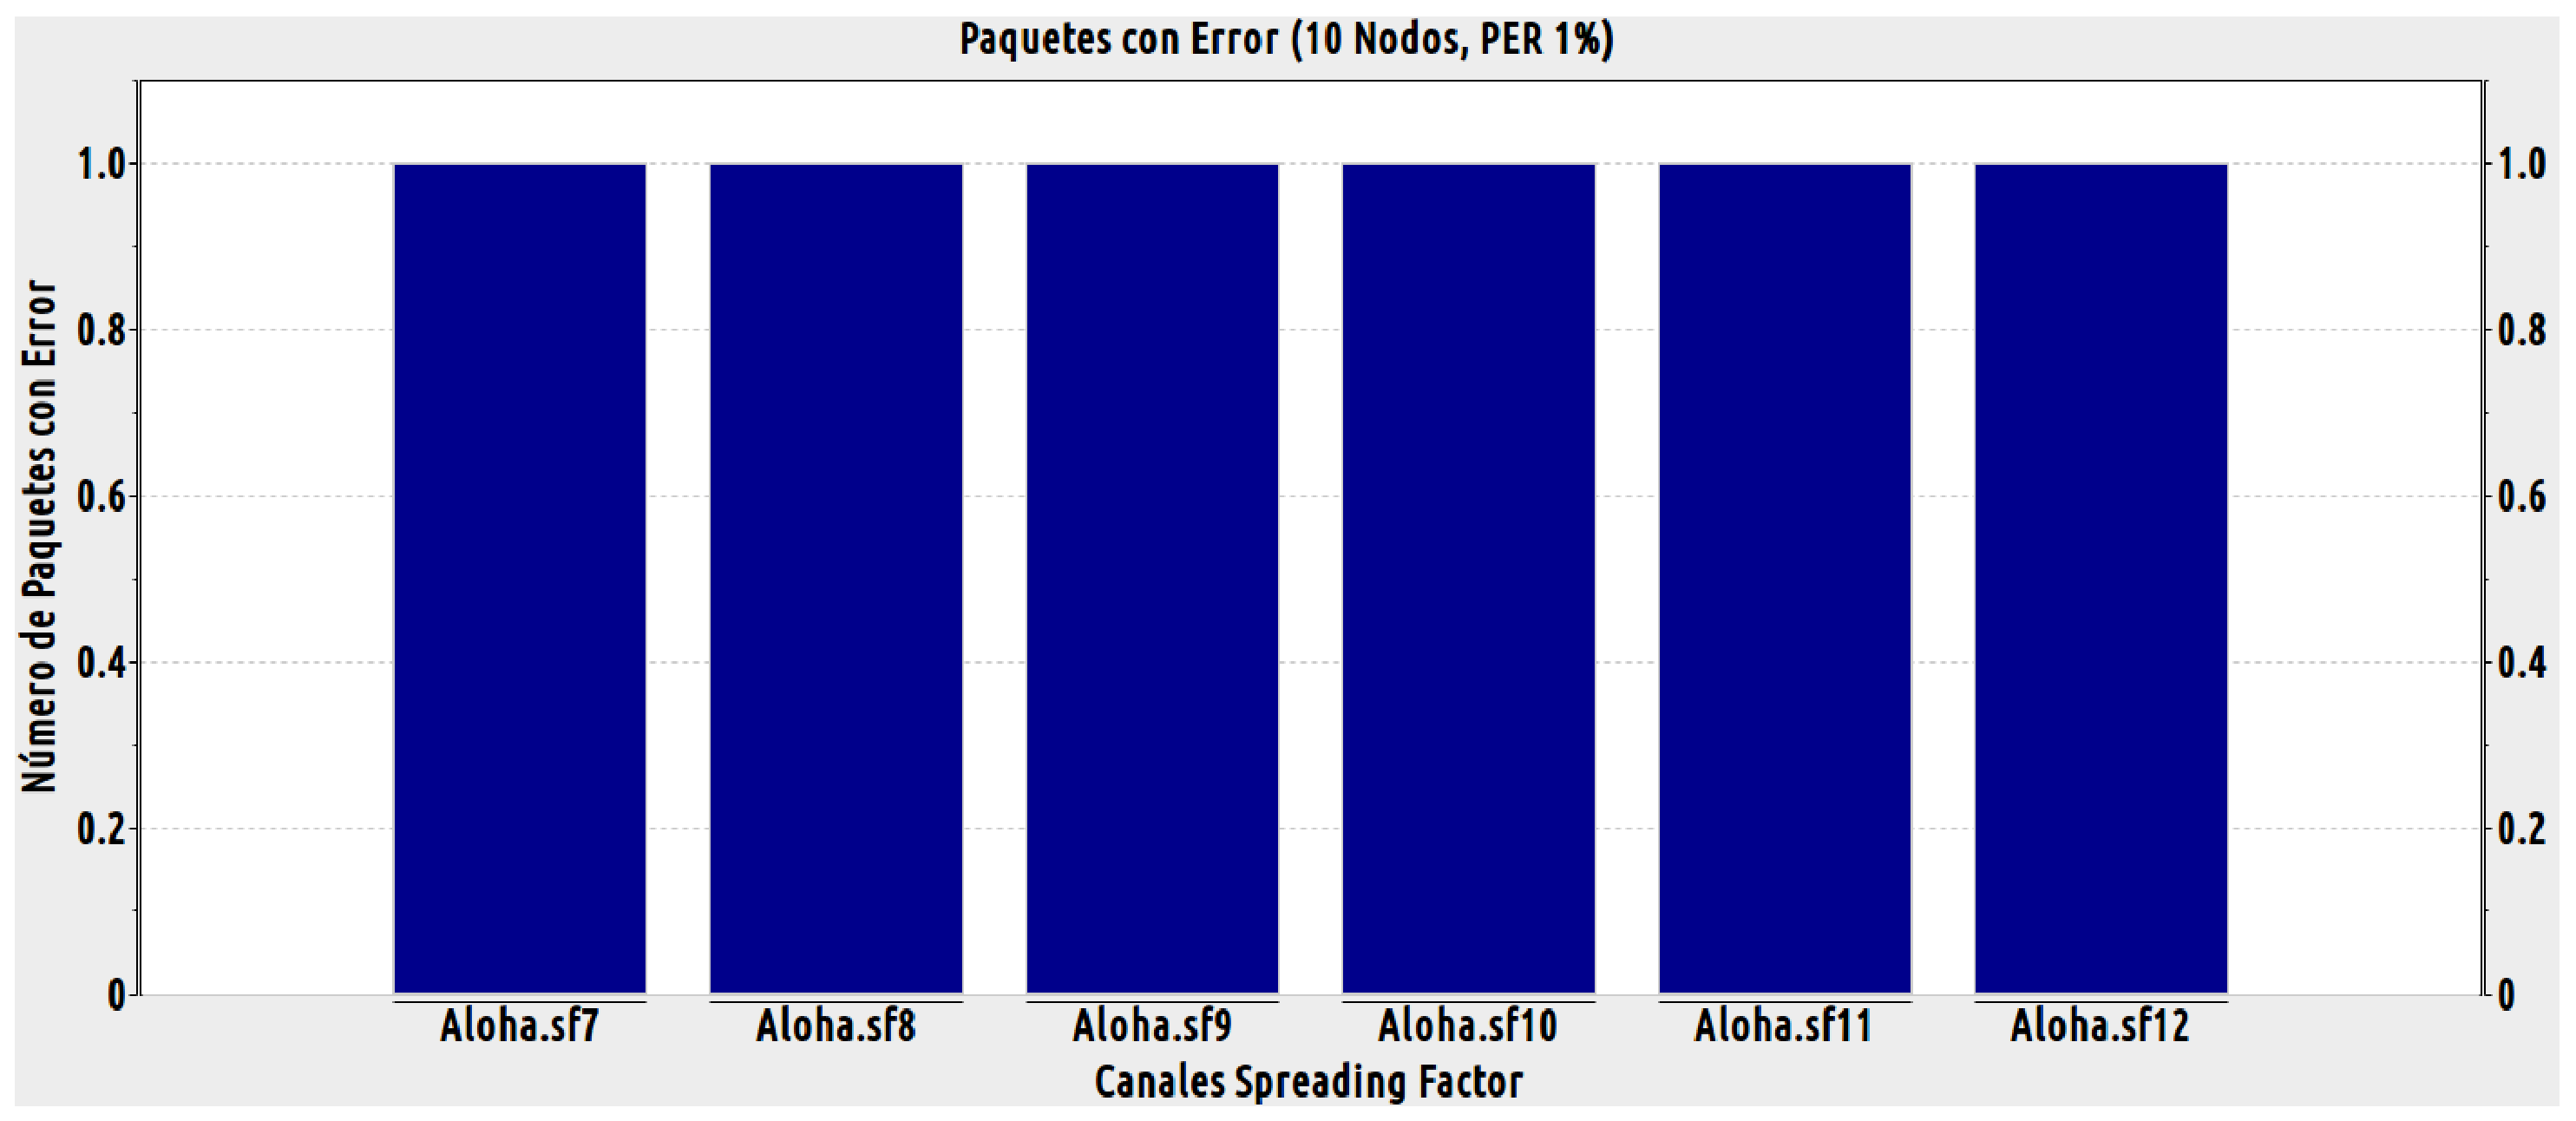
\includegraphics[width=13cm,height=30cm,keepaspectratio]{images/errores10nodos.eps}
\caption{Gráfico de cantidad de paquetes con errores en cada Spreading Factor en la simulación, para 10 nodos.\textit{Esta imagen puede verse ampliada en el Anexo~\ref{anexb:3}}}
\label{prueba:4}
\end{figure}
Sin embargo, en la Fig~\ref{prueba:5}, se evidencia un aumento considerable en la cantidad de paquetes con errores, donde la distribución ya no se hace tan homogénea como para el caso de diez nodos. Esto ocurre dado que por las colisiones y el orden arbitrario del simulador OMNET ++, algunos nodos pertenecientes a determinados Spreading Factor (en este caso particular, el SF8), poseen oportunidades más recurrentes de transmisión que otros, por lo que genera de que algunos Spreading Factor posean una cantidad menor del 1\%, que es esperable al, como también que en otros supere este 1\%. Este evento anómalo ocurre de forma análoga para la incongruencia en las colisiones para 100 nodos.\\
Este evento  es debido a que al momento de tomar el estado de la simulación, esta función no terminaba de acomodar el índice de paquetes con error al 1\%, ya que la función que calcula el índice de error en paquetes, a medida que llegan paquetes de forma íntegra al Spreading Factor este aumenta un contador de paquetes recibidos, por lo que al calcular el porcentaje de paquetes con error, este comienza a disminuir de forma constante, hasta que disminuye bajo el valor asignado de PER. Cuando esto ocurre, la función desecha el siguiente paquete en el Spreading Factor , aumentando con esto en uno el contador de paquetes con errores y por consecuencia el índice PER, donde nuevamente sigue calculando de forma cíclica hasta que el porcentaje disminuye hasta el valor asignado al PER. Este evento al no presentarse en todos los Spreading Factor por igual, no se atribuye una falla de diseño, o una falla del simulador, por lo que se presenta como anomalía que depende del tiempo cuando es detenida la simulación al momento de tomar datos estadísticos que representen el comportamiento de los dispositivos.\\
\begin{figure}[!ht]
\centering
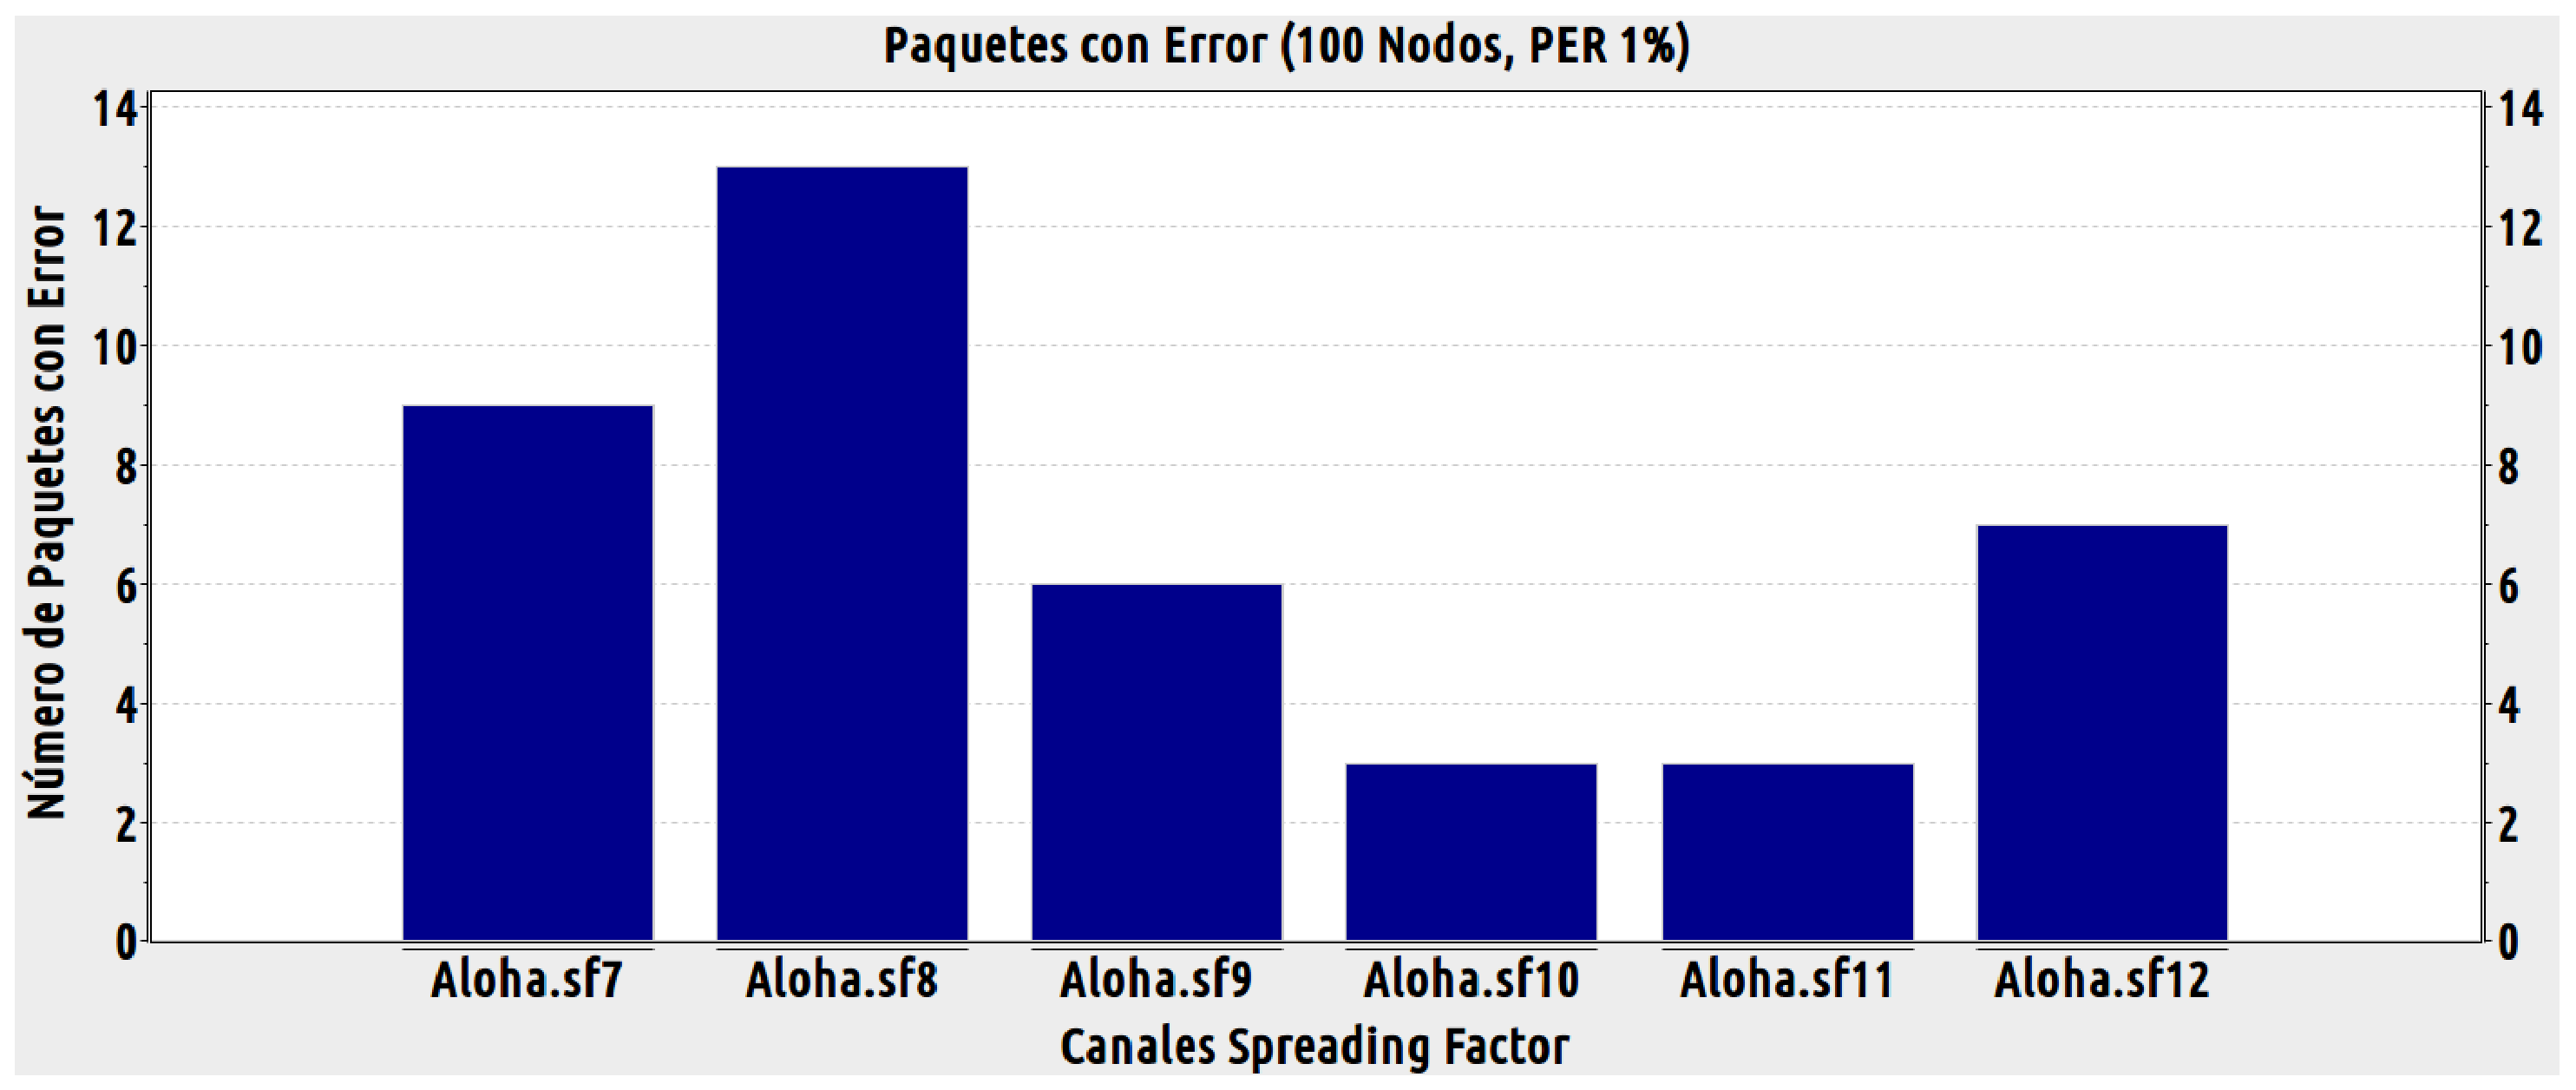
\includegraphics[width=13cm,height=30cm,keepaspectratio]{images/errores100nodos.eps}
\caption{Gráfico de cantidad de paquetes con errores en cada Spreading Factor en la simulación, para 100 nodos.\textit{Esta imagen puede verse ampliada en el Anexo~\ref{anexb:4}}}
\label{prueba:5}
\end{figure}
\end{justify}